\section{Q2: Who Is Hit Hardest?}
\label{sec:q2}

Fig.~\ref{fig:vuln} shows the causal forest for $Y_{\text{total}}$ on the 250 passive objects.
Drag sensitivity dominates the variable importance (0.892), well ahead of altitude (0.101) and
inclination (0.007), and the map barely changes across five forest seeds (minimum correlation
0.986). Seed stability tells us the algorithm is repeatable, not that the map would hold for new
storms. The first finding is no surprise given Eq.~\eqref{eq:drag}: in m/day, a large, light
object always loses more than a small, dense one.

The more interesting map is the effect per unit drag sensitivity (Fig.~\ref{fig:vuln}C). With
size divided out, altitude takes almost all the importance (0.993, against 0.005 for inclination
and 0.002 for drag sensitivity, with seed stability 0.995), and within each altitude row the map
is flat. So the storm effect is simply proportional to drag sensitivity, multiplied by an
altitude factor. That factor falls from $-10.8$ at 617~km to $-3.7$ at 747~km
((m/day per nT) per m$^2$/kg), about 2.9-fold over 130~km, or roughly one e-fold every
100--120~km. That is the same order as a thermospheric density scale height, which is a good sign
the map reflects real physics. As a cross-check, dividing the $Y_{\text{total}}$ map by drag
sensitivity cell by cell reproduces the per-drag forest (correlation 0.96). In this cohort,
inclination adds little once the response is averaged over an orbit.

The forest's intervals treat rows as independent, so we read the
map for its shape and take the size of the effect from DML. We do not interpret cells that rest
on a single group of objects (519 and 779~km).

\begin{figure*}[t]
\centering
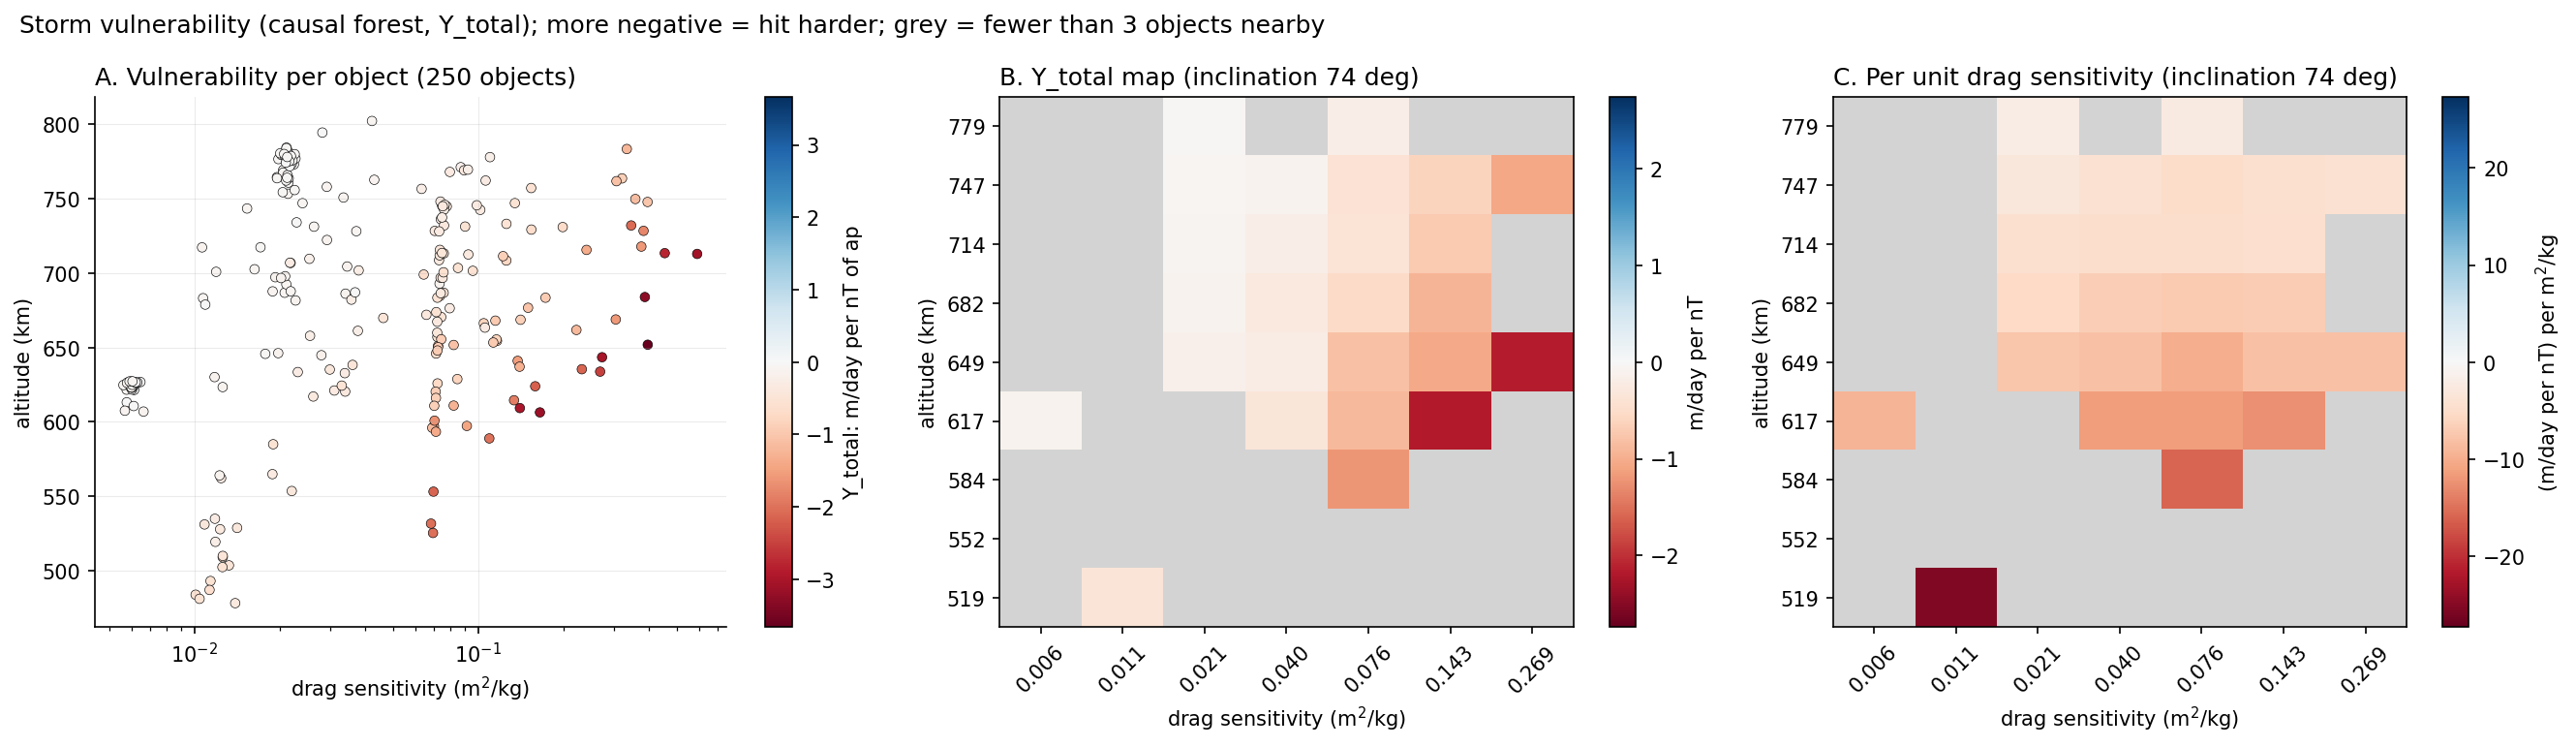
\includegraphics[width=\textwidth]{fig9_vulnerability.png}
\caption{Storm vulnerability (causal forest, 250 passive objects, m/day per nT of ap).
(A) Per-object effect. (B) Effect on an altitude $\times$ drag-sensitivity grid at the median
inclination. (C) Effect per unit drag sensitivity. Grey cells have fewer than three nearby
objects.}
\label{fig:vuln}
\end{figure*}
